\documentclass[a4paper,11pt,dvipdfmx]{ujarticle}
% パッケージ
\usepackage{graphicx}
\usepackage{url}
% レイアウト指定を記述したファイルの読み込み
\input{layout}

% タイトルと氏名を変更せよ.
\title{日本におけるデジタル化の状況}
\author{登内 凌汰}

\begin{document}

\maketitle %ここにタイトルが入る

% ここから本文
% 節見出し: \section{}
% を使う

\section{ブロードバンドの整理状況}


OECDによるブロードバンド回線に不急に関する調査\cite{oecd}によると,図\ref{fig:a}に示すように,
日本における100人あたりの光ファイバー回線の加入者数は29.0で,韓国,スウェーデン,ノルウェーに続いて第4位になっている.

\begin{figure}[htbp]
    \centering
    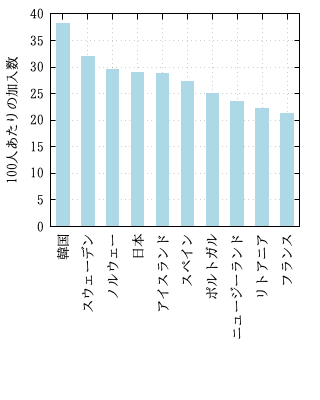
\includegraphics{fig11.png}
    \caption{光ファイバーの加入数(100人あたり)}\label{fig:a}
\end{figure}
% 本文(1)
%  参考文献の参照: \cite{}
%  図番号の参照: \ref{}
% を使う
% 文献データベースのキーワードは oecd と imd b
% になっている.

% 図の挿入
% \includegraphics{}
% を
% \begin{figure}[htbp]
% \end{figure}
% で囲み
% \caption{}
% で図のタイトルを入れる.
% \label{}
% を使って図番号が参照できるようにする
% また,
% \centering
% で図が中央に来るようにする

\section{デジタル競争力ランキング}

国際経済開発研究所(IMD)の調査\cite{imd}によると,
日本のデジタル競争力ランキングは表\ref{tbl:b}に示すように,
調査対象64カ国中,総合で28位,技術分野で30位となっている.

\begin{table}[htbp]
    \centering
    \caption{デジタル競争力ランキング(64カ国中)}\label{tbl:b}
    \begin{tabular}{|c|c|c|}
        \hline
        国 & 総合 & 技術 \\
        \hline
        米国 & 1位 & 4位 \\
        \hline
        香港 & 2位 & 10位 \\
        \hline
        スウェーデン & 3位 & 8位 \\
        \hline
        デンマーク & 4位 & 2位 \\
        \hline
        シンガポール & 5位 & 2位 \\
        \hline
        \hline
        韓国 & 12位 & 13位 \\
        \hline
        中国 & 15位 & 20位 \\
        \hline
        \hline
        日本 & 28位 & 30位 \\
        \hline
    \end{tabular}
\end{table}

    
% ーーー
% 節見出し(2)

% 本文(2)

% 表の挿入
% \begin{tabular}
% \end{tabular}    
% による表の記述を 
% \begin{table}[htbp]
% \end{table}
% で囲み
% \caption{}
% で表のタイトルを入れる.
% \label{}
% を使って表番号が参照できるようにする
% また,
% \centering
% で表が中央に来るようにする

\section{考察}

\begin{itemize}
    \item 日本はブロードバンドの整備状況では上位に入っており、通信インフラは充実している。しかし、それに比べてデジタル競争力のランキングが低いことから、インフラを活かしたイノベーションや人材育成が不足している可能性がある。
    \item 日本は技術的インフラは整っていても、それを活用するためのスキルや教育、ビジネスでの活用が他国に比べて遅れていると考えられる。デジタル人材の育成や企業のDX(デジタルトランスフォーメーション)推進が重要である。
    \item デジタル競争力を高めるためには、国内政策の見直しとともに、国際的な技術トレンドや基準への対応が必要である。日本独自のやり方に固執するのではなく、グローバルスタンダードを意識した取り組みが求められる。
\end{itemize}
% ーーー
% 見出し(3)
% 考察
%
% \begin{itemize}
% \end{itemize}
% を使って箇条書きで記述する


% ここに参考文献が入る
%
\bibliographystyle{junsrt}
\bibliography{exercise.bib}

\end{document}